\chapter{Project Design} %TODO

\section{Overall Architecture}

schema

\section{Database}

\paragraph{}
We searched for already created database with some test data that can be publicly used but we didn’t have luck. So we were forced to create our own database.\\
The database technology that we decided to use is PostgreSQL (https://www.postgresql.org/).\\
The software is open-source, which means that the source code is available at no charge. In that way if we have a need to customize or extend PostgreSQL in any way then we are able to do so with a minimum of effort, and with no attached costs.\\
PostgreSQL is available for almost every brand of Unix (34 platforms with the latest stable release), and Windows compatibility is available via the Cygwin framework.\\
And last but not least, the legendary reliability and stability of PostgreSQL.

In the area of medicine and health care it is a well known fact that there is a lot of data and many different aspects that can be considered, when taking a decision or making a diagnosis. \\
After analyzing the data itself we decided that we will choose the relational data model.
The reason is that we have a lot of data that can be dependent upon other data.\\
One obvious and clear example of that is the disease’s dependency upon symptom(s).\\
\\
Example : 
Let’s imagine that someone has the following symptoms : high temperature, fever, cough, tiredness and sweating. 
Obviously, assuming all of those symptoms we can conclude that the person might has flu. But if the person was complaining about low temperature instead of high temperature, we would most likely assume pneumonia as a state of the condition. The reason is that low temperature combined with the other symptoms is more typical for pneumonia than flu. 
Both of the examples show how we can differ our decisions one from another and how we make decision according to the chosen decision-making strategy. In other words diagnosis or more specifically final disease is the decision and the symptoms are defining our basic decision-making strategy.\\
\\
High temperature, fever, cough, tiredness, sweating → Flu\\
Low temperature, fever, cough, tiredness, sweating → Pneumonia\\
\\
Basic decision-making strategy : Symptoms\\
Decision : Diseases\\
\\
There is alternative interpretation that is valid for the upper case. The inverted case.
We can say that we can invert the roles and we will still have true logic.\\  
So we will have this :\\
\\
Flu $\rightarrow$ High temperature, fever, cough, tiredness, sweating \\
Pneumonia 		$\rightarrow$	  Low temperature, fever, cough, tiredness, sweating\\
\\
Basic decision-making strategy : Diseases\\
Decision : Symptoms\\
\\
To summarize we can say that the data dependency is bidirectional.\\
\\
Flu $\leftrightarrow$ High temperature, fever, cough, tiredness, sweating\\
\\
This is leading to the biggest problem – data handling.
In other words  we are forced to use many-to-many relationship model which is leading to a difficulties in data inserting and Big Data.

\section{Database structure and design}
\paragraph{}

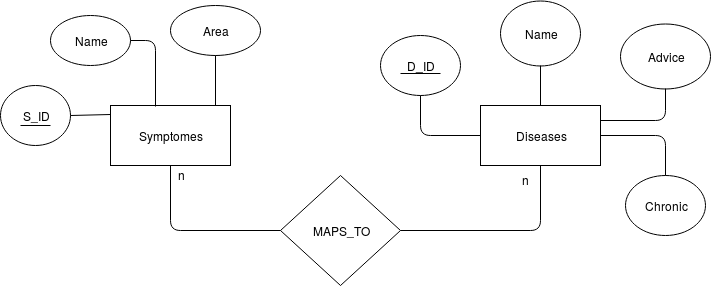
\includegraphics[height = 0.35\textheight, width = \textwidth]{DB}

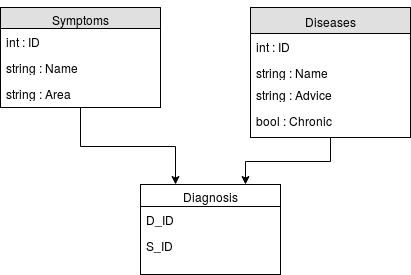
\includegraphics[height = 0.35\textheight, width = \textwidth]{UML}
\\
\\
\section{Data model}
\paragraph{}
We have 3 tables in our relational database.\\
\\
Symptoms – id, name and area which the symptom occurs. \\
Diseases – id, name, advice (medical advice if you are in that condition), chronic(boolean value used to show us if the disease is chronic or not)\\
Diagnosis – table connecting the symptoms with the diseases by ids.\\

A problem that occur our project is finding trustworthy data.\\
The data we are using is taken from http://www.mayoclinic.org/ .\\ 
The development team of the website consists of experts in the medical field. 
Physicians, scientists and other medical experts contributed to the website with their knowledge and experience. That’s the main reason why we decided to trust this website and use the data from it.   

As you can see from the diagrams the database is complicated when it’s about inserting data in it.
With the current design and structure it’s impossible to be done join between the tables for symptoms and diseases because of the data dependency. In a result while inserting data, every time we should fill the data manually in the diagnosis table in order to have the connection between every symptom and disease at the end. 
The other problem that is occurring is that the more data we are inserting the bigger becomes the diagnosis table. That means that at some point we are going to face the big data problem.

